\documentclass{sigchi}

% Load basic packages
\usepackage{balance}  % to better equalize the last page
\usepackage{graphics} % for EPS, load graphicx instead 
\usepackage{mathptmx}
\usepackage[pdftex]{hyperref}
\usepackage{color}
\usepackage{booktabs}
\usepackage{textcomp}
\usepackage{microtype} % Improved Tracking and Kerning
\usepackage{ccicons}  % Cite your images correctly!
\usepackage{multicol}
\usepackage{color} 
\newcommand{\hl}[1]{\colorbox{yellow}{#1}}
\usepackage{xspace}
\usepackage{algorithm} 
\usepackage{algpseudocode} 
\usepackage{subcaption}
\usepackage{booktabs}
\def\algname{SPRING\xspace}
\DeclareMathOperator*{\argmin}{argmin}
\DeclareMathOperator*{\argmax}{argmax}

\floatname{algorithm}{Procedure}
\renewcommand{\algorithmicrequire}{\textbf{Input:}}
\renewcommand{\algorithmicensure}{\textbf{Output:}}


\usepackage{tikz}
\usetikzlibrary{decorations.pathreplacing,calc}
\newcommand{\tikzmark}[1]{\tikz[overlay,remember picture] \node (#1) {};}
\newcommand*{\AddNote}[4]{%
    \begin{tikzpicture}[overlay, remember picture]
        \draw [decoration={brace,amplitude=0.2em},decorate, thick, darkgray]
            ($(#3)!(#1.north)!($(#3)-(0,1)$)$) --  
            ($(#3)!(#2.south)!($(#3)-(0,1)$)$)
                node [align=center, text width=2.5cm, pos=0.5, anchor=west] {#4};
    \end{tikzpicture}
}%


% Paper metadata (use plain text, for PDF inclusion and later
% re-using, if desired).  Use \emtpyauthor when submitting for review
% so you remain anonymous.
\def\plaintitle{A Data-Driven Approach for Inferring Student Proficiency from Game Activity Logs  }
\def\plainauthor{Mohammad H. Falakmasir, Jos\'{e} P. Gonz\'{a}lez-Brenes, Geoffrey J. Gordon, Kristen E. DiCerbo}
\def\emptyauthor{}
\def\plainkeywords{Authors' choice; of terms; separated; by
  semicolons; include commas, within terms only; required.}
\def\plaingeneralterms{Documentation, Standardization}


% llt: Define a global style for URLs, rather that the default one
\makeatletter
\def\url@leostyle{%
  \@ifundefined{selectfont}{
    \def\UrlFont{\sf}
  }{
    \def\UrlFont{\small\bf\ttfamily}
  }}
\makeatother
\urlstyle{leo}

% To make various LaTeX processors do the right thing with page size.
\def\pprw{8.5in}
\def\pprh{11in}
\special{papersize=\pprw,\pprh}
\setlength{\paperwidth}{\pprw}
\setlength{\paperheight}{\pprh}
\setlength{\pdfpagewidth}{\pprw}
\setlength{\pdfpageheight}{\pprh}

% Make sure hyperref comes last of your loaded packages, to give it a
% fighting chance of not being over-written, since its job is to
% redefine many LaTeX commands.
\definecolor{linkColor}{RGB}{6,125,233}
\hypersetup{%
  pdftitle={\plaintitle},
% Use \plainauthor for final version.
%  pdfauthor={\plainauthor},
  pdfauthor={\emptyauthor},
  pdfkeywords={\plainkeywords},
  bookmarksnumbered,
  pdfstartview={FitH},
  colorlinks,
  citecolor=black,
  filecolor=black,
  linkcolor=black,
  urlcolor=linkColor,
  breaklinks=true,
}

% create a shortcut to typeset  headings
% \newcommand\tabhead[1]{\small\textbf{#1}}

% End of preamble. Here it comes the document.
\begin{document}

\title{\plaintitle}

\numberofauthors{4}
\author
{%
  \alignauthor{\mbox{\hspace{-1.85em}Mohammad H. Falakmasir$^{\star, \#} $\;\;\; Jos\'{e} P. Gonz\'{a}lez-Brenes$^\star$ \;\;\; Geoffrey J. Gordon$^\S$ \;\;\; Kristen E. DiCerbo$^\star$}\\
    \affaddr{$^\star$School Research}\\
    \affaddr{Pearson}\\
    \email{\{jose.gonzalez-brenes, kristen.dicerbo\}@pearson.com }\\
    }
  \alignauthor{\vphantom{Mohamamad Jose}
    \affaddr{$^\#$Intelligent Systems Program} \\
    \affaddr{University of Pittsburgh}\\
    \email{falakmasir@pitt.edu}\\
  }
  \alignauthor{\vphantom{Mohamamad Jose}
  	\affaddr{$^\S$Machine Learning}\\
	\affaddr{Carnegie Mellon University} 
  	\email{ggordon@cs.cmu.edu}\\
  }
}

  
\maketitle

\begin{abstract}
Traditional assessments are important in education because they allow collecting evidence about student progress. 
Unfortunately, they can be very tedious to their stakeholders.
In contrast, invisible assessment  unobtrusively gathers  performance data from students' daily activities to make inference about student relevant competencies.
We present a novel data analysis pipeline, {Student Profficiency Inferrer from Game data} (\algname), that allows modeling  game playing behavior in educational games.
Unlike prior work, \algname is a fully data-driven method that does not require costly domain knowledge engineering.
We validate our method using data collected from students playing 11 educational mini-games.
Our results suggest that  \algname is accurate to predict Math assessments ($R^2$ =0.55 , Spearman $\rho$=0.82).
%We provide insights in how to use \algname to understand student exploration habits, misconceptions, and how to improve the game design based on their playing strategies.
\end{abstract}

\category{K.3.1}{Computer Uses in Education.}
{}
\keywords{Educational Games, Student Modeling, Stealth Assessment}

\section{Introduction}
Educational assessments are important because they collect evidence about about  whether  the teaching goals are being met or not.
Unfortunately, the process of  administering assessments is usually disconnected from the learning environment, and  it is often  disruptive to the classroom. 
In many developed countries, students now find themselves spending increasing amounts of time preparing and taking tests instead of learning~\cite{hofman2015rebalancing}.
For example, a  survey of the current state of testing in America revealed that students are taking an average of 113 standardized tests between pre-K and highschool~\cite{lazarin2014testing}. 
For these reasons, it is not surprising that the recent political climate and the general population have been weighing in on the question of whether students are being tested too much~\cite{lazarin2014testing}.


According to Evidence Centered Design (ECD)~\cite{mislevy2012design}, the goal of assessment is to characterize the strength of evidence regarding claims one wants to make about individuals or groups.
Therefore, the assessment process involves identifying, organizing, or creating activities for students so we may observe that evidence.
An interesting alternative to traditional summative assessment is invisible (or stealth) assessment~\cite{shute2013stealth},
where the evidence is gathered from leaners unobtrusively from the digital interactions of their ongoing activities.
This data is used  to understand claims regarding what students know and what they can do \cite{shute2009melding}.
Stealth assessment is also intended to reduce or eliminate test anxiety, while not sacrificing validity and reliability \cite{shute2008you}.



A promising opportunity for invisible assessment is using log data collected from educational games.
Unfortunately, engineering a system that parses log data is costly and time-consuming.
For example, prior work~\cite{shute2013stealth, shute2009melding} has relied extensively on subject matter expertise to define a \textit{Competency Model} in form of a Bayesian Network to describe the set of knowledge and skills involved in the learning environment.
They also used feature engineering on the performance data to build an \textit{Evidence Model} that expresses how student interactions with the system constitute evidence about competency model variables.

Our motivation is that invisible assessment from game data may become more accurate and cheaper to implement if the domain knowledge engineering could be automated by a data-driven process.
Game data is often logged  in a format that we call a \textit{slot and filler} structure.
In Table~\ref{tbl:log_example}, we show a simplified example of a real educational game log that uses slot and filler structure.
The slots are discrete sets of events that are initiated by the leaner.
Each slot may accept zero to multiple fillers. 
Each filler represents a value of a property of the slot event.
For example, a \texttt{Move Object} event  that represents the learner moving an object in the screen, may have an $x$ and $y$ coordinates as fillers to represent the target position in two-dimensional space.

\begin{table}[tbh]
	\begin{tabular}{@{}llll@{}}
		\toprule
		\textbf{Id}             & \textbf{User Id} & \textbf{Event Name} & \textbf{Event Data}        \\ \midrule
		1                       & ABC              & Game Start          & \{ \}                        \\
		2                       & ABC              & Move Object         & \{X:363,Y:82\} \\
		3                       & ABC              & Move Object         & \{X:361,Y:54\} \\
		4                       & ABC              & Open Toolbox        & \{\}        \\
		4                       & ABC              & Activate Tool        & \{tool:gluumi\}        \\
		5                       & ABC              & Use Gluumi        & \{sizeGluedTo:8,sizeNew:9\} \\        
		\multicolumn{1}{c}{...} &                  &                     &                            \\ \bottomrule
	\end{tabular}
	\caption{An example fragment of a log from an educational game. \label{tbl:log_example}}
\end{table}

Conventional machine learning algorithms cannot input slot and filler data, as they usually work with structures such as  \textit{feature vectors} and \textit{sequences}.
Prior work~\cite{sequences} provides a   review of  the difference between feature vectors and sequences.
A feature vector representation requires mapping an observation onto a fixed number of features.
It is not trivial to map sequences of student actions that can be of an arbitrary length into a feature vector that needs to be of a predetermined dimension.
Traditional feature vector classifiers,  like logistic regression or decision trees,  that are used in off-the-shelf data mining packages, such as Weka \cite{hall2009weka}, cannot  use slot and filler data as input. 
In contrast, machine learning algorithm that allow sequential representations, like Hidden Markov Models (HMM), require a parametric model with the same number of dimensions for all of the observations.
This does not occur in slot and filler structures.
For example,  in Table~\ref{tbl:log_example}, the \texttt{Move Object} slot requires \texttt{x} and \texttt{y} fillers, while the \texttt{Use Gluumi} slot requires \texttt{size} fillers.

In this paper, we propose \textit{Student PRofficiency INferrer from Game data} (SPRING), a novel data analysis pipeline that models game playing behavior.
\algname allows modeling raw data in slot and filler structure.
We demonstrate our approach on real student game playing data.
Our experiments suggest that \algname can be used to predict student proficiency  without costly domain expertise.

\section{SPRING Framework}

\algname is designed in a way that can capture sequential decision making process of students in a way that is representative of their mastery with minimum reliance on expert knowledge. Our data analysis pipeline receives raw data of student interactions with the different levels of educational game in slot and filler format along with their post-test results and creates a regression model for predicting the post-test scores. 
Algorithm~\ref{alg:spring} describes the three main steps of our pipeline: discretization,  sequence modeling, and regression.
The discretization step transform slot and filler observations into multinomial indicators that are used as evidence for learning.
The sequence modeling step, learns a representation from data in form of a Hidden Markov Model for high- and low-performing students.
The regression step, uses the likelihood of student sequences in each game level as a feature to predict the post-test results.
We now explain the different steps in detail.

\begin{algorithm}
\begin{algorithmic}[1]
\Require: A log file $\mathbf{L_{g,s}}$ of slot-and-filler structure for each game $g$ and student $s$, a test $y_s$ for each student
\For {each  game $g$}  \tikzmark{sectop}
\State $\mathbf{D_{g,s}} \leftarrow$  Discretize($\mathbf{L_{g,s}}$) \tikzmark{discbot}
\State  $\langle \mathbf{High_{g}} , \mathbf{Low_{g}} \rangle \leftarrow$  Cluster\_Students($\mathbf{D_{g,s}}, y_s$) \tikzmark{disctop}\tikzmark{right}\tikzmark{secright}
\State$\theta_{h,g} \leftarrow$  Learn\_HMM($ \mathbf{High_{g}} $)
\State$\theta_{l,g} \leftarrow$  Learn\_HMM($ \mathbf{Low_{g}} $)
\For{each sequence $d$ in $\mathbf{D_{g,s}}$}
\State  $\phi_{g,s} \leftarrow$  Extract\_Features($d,\theta_{h,g}, \theta_{l,g}$) 
\EndFor
\EndFor \tikzmark{secbot}
\State Predict $y_s$  from $\phi_{g,s}$ \tikzmark{regtop}
\tikzmark{regbot}
\end{algorithmic}
\caption{The SPRING algorithm\label{alg:spring}}
\end{algorithm}



\subsection{Discretization}
\hl{Each section should refer to line numbers in the algorithm}
\hl{Make sure the notation is consistent between algorithm and steps}
This step of the data analysis pipeline receives time-stamped student interactions in slot and fillers format as input and generates a sequence of multinomial observations for each student in each game level.
In order to transform the slot and filler observations into multinomial, we use DBSCAN clustering algorithm \cite{ester1996density} on the filler dimensions. 
We tried different unsupervised and non-parametric methods, however, we ended up using DBSCAN because it can find arbitrarily shaped clusters and does not require one to specify the number of clusters in the data a-priori.
It is also robust to outliers which in our case can be considereded as noisy movements that are not representative of learning competency. 
We considered outliers as a separate cluster assuming that movements outside high density regions are either occure because of technical glitches in the gaming environent or misconceptions that are not common across multiple students. 

Figure~\ref{fig:figurecluster} shows an example of using clustering to discretize \texttt{Move Object} slots, that have $x$ and $y$ coordinates as fillers.
Figure~\ref{fig:screenshot} shows a screenshot of one of the game levels where students have to move ice cubes from the mountain top onto the two designated areas to prevent the yeti from crossing the wall.
Figure~\ref{fig:clustering} shows a scatterplot of the $x$ and $y$ fillers of student movements along with clusters detected.
We colored the points according to the DBSCAN clustering.
In this example, we have three clusters,  cluster one and two (red and yellow respectively) that represent the frequent movements, and cluster zero (black) that represents outlier movements.

\begin{figure}[t]
 \centering
\begin{subfigure}{.5\textwidth}
	\centering
	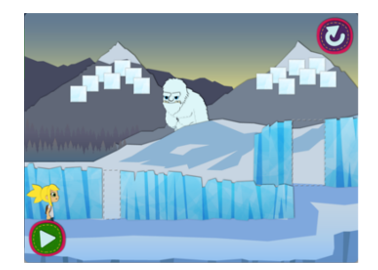
\includegraphics[width=0.9\columnwidth]{figures/glacier_screenshot.png}
	\caption{Screenshot of game level 2, \textit {None Shall Pass!} \label{fig:screenshot}}
\end{subfigure}
\begin{subfigure}{.5\textwidth}
	\centering
	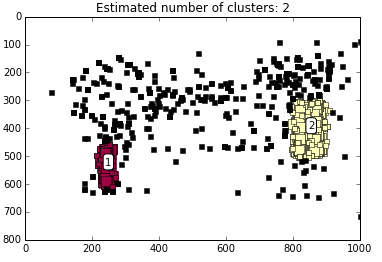
\includegraphics[width=0.9\columnwidth]{figures/glacier_positions.png}
	\caption{Clusters detected among student movements in game level 2 \label{fig:clustering}}
\end{subfigure}
\caption{The clusters detected for game level 2, \textit {None Shall Pass!}, using DBSCAN method. We transform each movement action into corresponding cluster id during the discretization step.\label{fig:figurecluster}}
\end{figure}

After running DBSCAN on the filler dimensions, we trained a K-Nearest Neighbor (K-NN) Classifier on the fillers and cluster labels. 
Tha main reason for training the classifier was that the default implementation of DBSCAN only returns cluster labels for the points in its dataset. 
However, our discretization phase should be able to transform any unseen fillers into a cluster label. 
K-NN classifier was a good candidate for this phase because both K-NN and DBSCAN use euclidean distance as a metric to evaluate the distance between the points. 
We used this classifier to  extract the cluster label for any  filler and we use the concatanation of slot and cluster labels as a multinomial observation in the sequence modeling phase.
The details of the discretization phase is demonstrated in Procedure~\ref{alg:discretize}.
\hl{Show an example input (slot-filler), and an example output (discrete sequence) to help illustrate the point}

\begin{algorithm}
	\begin{algorithmic}[1]
		\Require: $S_g$, Sequence of slot-and-filler observations in game level $g$
		\Procedure{Discretize}{S}
		\State{A = empty dictionary of slots and possible fillers}
		\For{each sequence s in S }
		\For{each action a in s}
		\If{a.filler $\neq \varnothing$}
		\State{A[a.slot].append(a.filler)}
		\EndIf
		\EndFor
		\EndFor
		\State
		\For{each slot and fillers tuple in A}
		\State{clustersIDs = DBSCAN(a.fillers)}
		\State{$C_s$ = K-NN classifier on fillers and clusterIDs}
		\EndFor
		\State
		\State{D = [][]\textit{ --2D array of multinomial observations}}
		\For{each sequence $seq$ in $S$}
		\For{each slot and filler tuple $\langle s, f \rangle $ in $seq$}
		\State{$D_{i,j}$ = $C_s$.predict($f$)}
		\EndFor
		\EndFor
		\State \Return{D}
		\EndProcedure
		
	\end{algorithmic}
	\caption{The Discretization Step of \algname \label{alg:discretize}}
\end{algorithm}



\subsection{Sequence Modeling}
Hidden Markov Models are good a candidate for the task of unsupervised analysis of sequential data.
The use of hidden Markov models for clustering sequences appears to have first been mentioned in \cite{juang1985probabilistic} and subsequently used in the context of discovering subfamilies of protein sequences \cite{krogh1994hidden}. 
However, it is important to note that the motivation for our framework comes from the goal of learning a \textit{descriptive} model from the data, rather than a \textit{predictive} model.
Given the sequence of student actions, we aim to infer meaningful sequence of (latent) states, which describe the process that generated the actions, along with statistical patterns that can describe and distinguish those states.
\hl{Moreover, we need states that represent meaningful patterns among students using a clustering method}

Learning the ``best" value for number of clusters ($K$) is a difficult problem in practice even for non-dynamic models. 
There has been considerable prior work on this problem that used penalized likelihoods \cite{rabiner1989hmm}, Monte-Carlo cross-validation \cite{smyth1996clustering}, and mixture of HMMs \cite{smyth1997clustering}. 
However, for simplicity purposes, we hypothesized that high- and low-performing students have similar usage patterns that are representative of their sequential decision-making process. Instead of learning the number of clusters from data, we used the post-test scores to divide students into two groups and learned a HMM for each group.

We used the Hierarchical Diriclet Process HMM (HDP-HMM) \cite{fox2008hdp}, which is allows state spaces of unknown size to be learned from data. 
HDP-HMM defines a \textit{hierarchical Dirichlet process} prior on transition matrices over countably infinite state spaces and is able to make a principled choice of how many states it needs based on the complexity of its training data. 
For details on training methods please refer to \cite{fox2008hdp}.

We used the output of the discretization step (2D array of multinomial observations) and trained two HDP-HMMs, one for high-performing and the other for low-performing students in each game level. The two models can be considered as a stochastic representation of the sequence of actions and we can use them to infer the likelihood of any arbitrary sequence as a feature for the regression step. 

\subsection{Regression}

%In this phase, we created a linear regression model using the likelihoods extracted from the previous phase. 
For each student $s$  in each game level $g$, we calculate the difference ($d_{s,g}$) of the likelihood of belonging to high performing group minus the likelihood of of belonging to the low performing group.
We calculate this likelihood by estimating the Forward-Backward probabilities  on each student sequence sequence of actions  based on the two HMMs parameter we estimated (whether the student is in the high performing group or in the low performing group):
\begin{equation}
d_{s,g} = \theta_{g, \text{high}} - \theta_{g, \text{low}}
\end{equation}

We use  a linear regression model for predicting the post-test scores:

\begin{equation}
\hat {y_s}(\beta) =   \sum_g \beta_g \cdot d_{s,g}  + \beta_0
\end{equation}

Here, $\beta_0$ is just an intercept for the  model.  
We optimized the parameters of the model using a 5-fold cross validation on our development set.
We experimented with different regularization methods, but only report LASSO \cite{tibshirani1996regression} as it worked best in our preliminary comparisons:
\begin{equation}
\beta^* = \argmin_\beta || y_s - \hat{y_s}(\beta)  ||_2 + \lambda \cdot || \beta ||_1
\end{equation}


\section{Empirical Evaluation}

\subsection{Game Environment}
\textit {Alice in AreaLand} is an educational game developed for research purposes. It focuses on teaching and assessing geometric measurement, specifically the understanding of area, among 6\textsuperscript{th} grade students. The game targets three main stages in the development of area: 1) area unit iteration, 2) use of unit squares to measure area, and 3) use of composites to measure area. The current version has 11 game levels. A simple student scenario involves covering a 2D area with smaller unit squares placed end-to-end in non-overlapping fashion, combining the single squares into rows or columns, and then determining the number of rows or columns needed. Figure~\ref{fig:figurekracken} shows a screenshot of one game level.

\begin{figure}
	\centering
	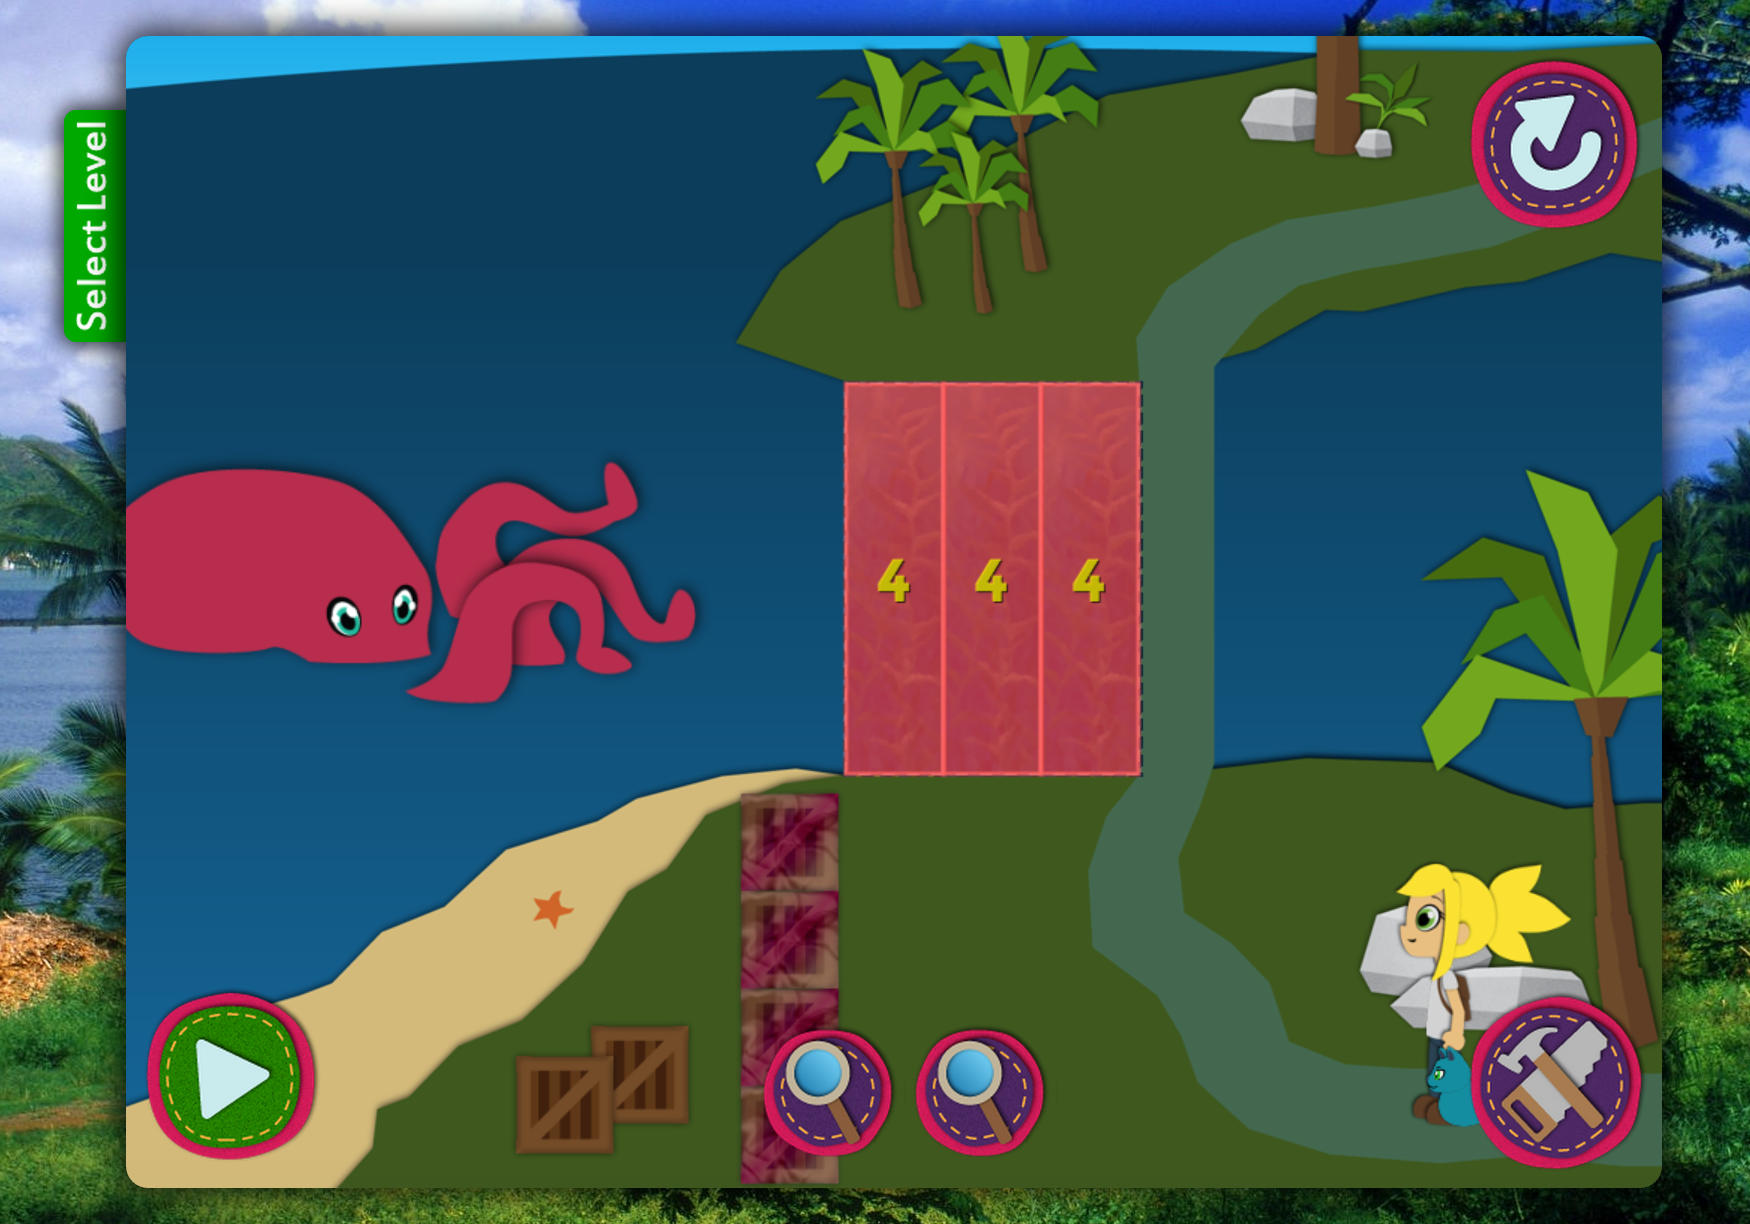
\includegraphics[width=0.9\columnwidth]{figures/kracken}
	\caption{A screenshot of hint provided in game level 11, \textit {You Kraken Me Up!}, in \textit {Alice in AreaLand}. Students should combine four squares into a column and create three copies of the column to cover the designated area and prevent the octopus from attacking \textit {Alice} while she crosses the bridge.}~\label{fig:figurekracken}
\end{figure}

Throughout the game,  \textit {Alice} is accompanied by \textit {Flat Cat} -- an assistant character who provides feedback and scaffolding to the player in the beginning of each game level and upon request when students push a hint button (represented by two magnifiers at the bottom center of Figure ~\ref{fig:figurekracken}). Earlier game levels are designed for students to learn about area unit iteration and usually require them to cover a number of predefined areas with unit squares (not necessarily in a non-overlapping fashion). By advancing through game levels, students are presented with three tools: \textit {Gluumi} for combining unit squares by gluing them together; \textit {Multy}, for making copies of different objects; and \textit {Esploda} for breaking compound shapes into single units.  There is no limit for completing a game level regarding time or number of actions students may execute. The students press the \textit {Go Alice} button (bottom left corner of Figure~\ref{fig:figurekracken}) if they deem their performance to be satisfactory for \textit {Alice} to proceed. Based on the covered area and the arrangement of the tiles, they either advance to the next level or receive a feedback and stay in the same level.

\subsection{Dataset} 
Our dataset consists of time-stamped interactions of 129 students in 11 game levels. 
For 77 students, we also have post-test scores from a paper-based exam with 20 questions in the 3 skills of geometric measurement.
In total, there are 88,458 events recorded in the dataset from 1,510 game sessions, meaning that student tried some of the game levels for multiple times.
Based on the ECD framework, beginning levels only involve area unit iteration skill and the other skills and related features are gradually added to the later game levels.
Figure \ref{fig:frequency} shows the frequency of different events in each game level. As depicted in Figure \ref{fig:frequency}, the student interactions with the system in all game levels is dominated by movements.

\begin{figure}
	\centering
	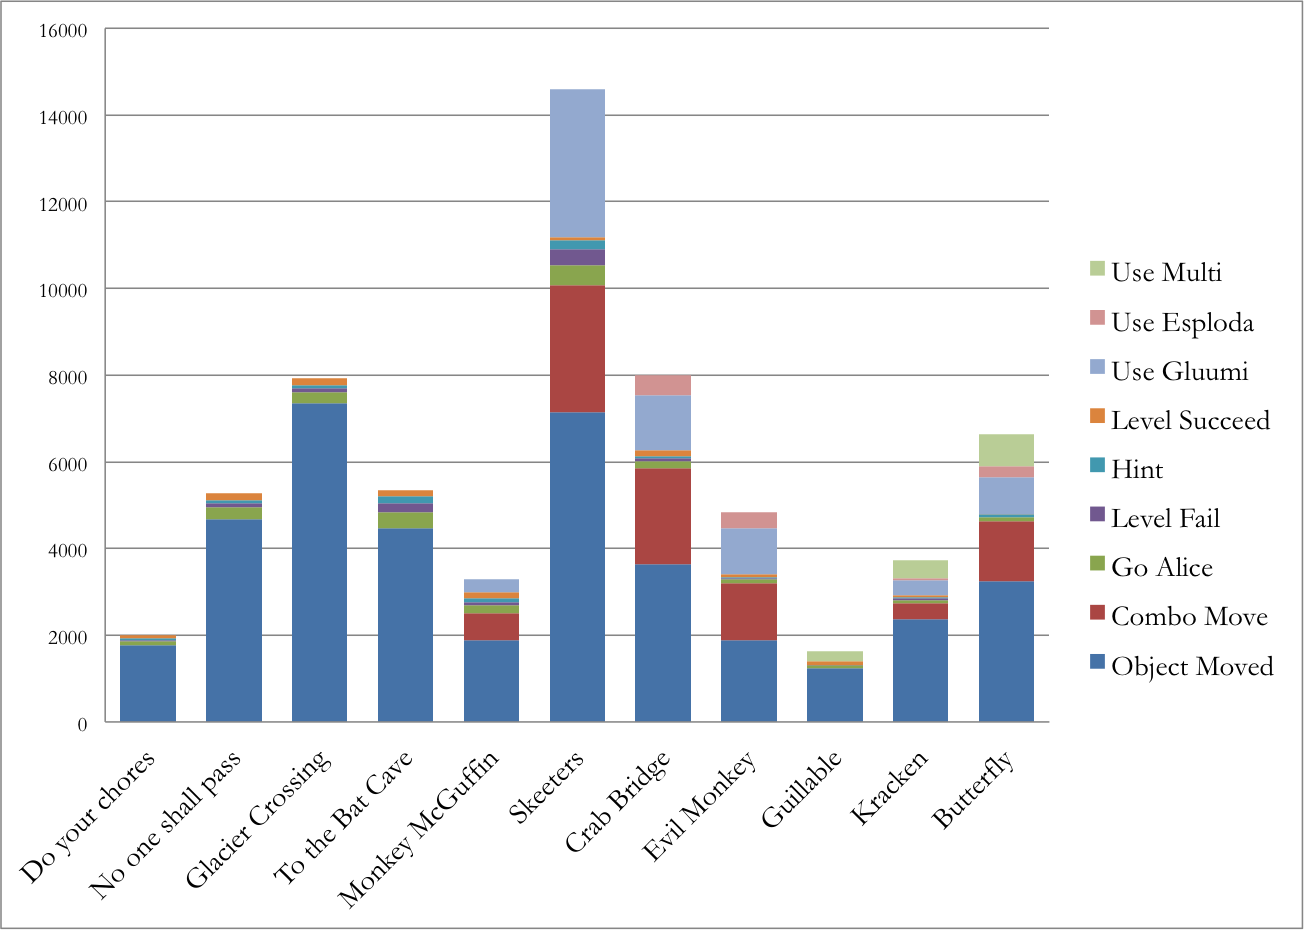
\includegraphics[width=0.9\columnwidth]{figures/frequency}
	\caption{Frequency of Events in Each Game Level}~\label{fig:frequency}
\end{figure}

We only used the interactions of the students who participated in the post-test.
In the case of multiple attempts in a game level, we only considered the interactions from the first attempt.
Figure \ref{fig:boxplot} shows the boxplot of sequence length in each game level. 

\begin{figure}
	\centering
	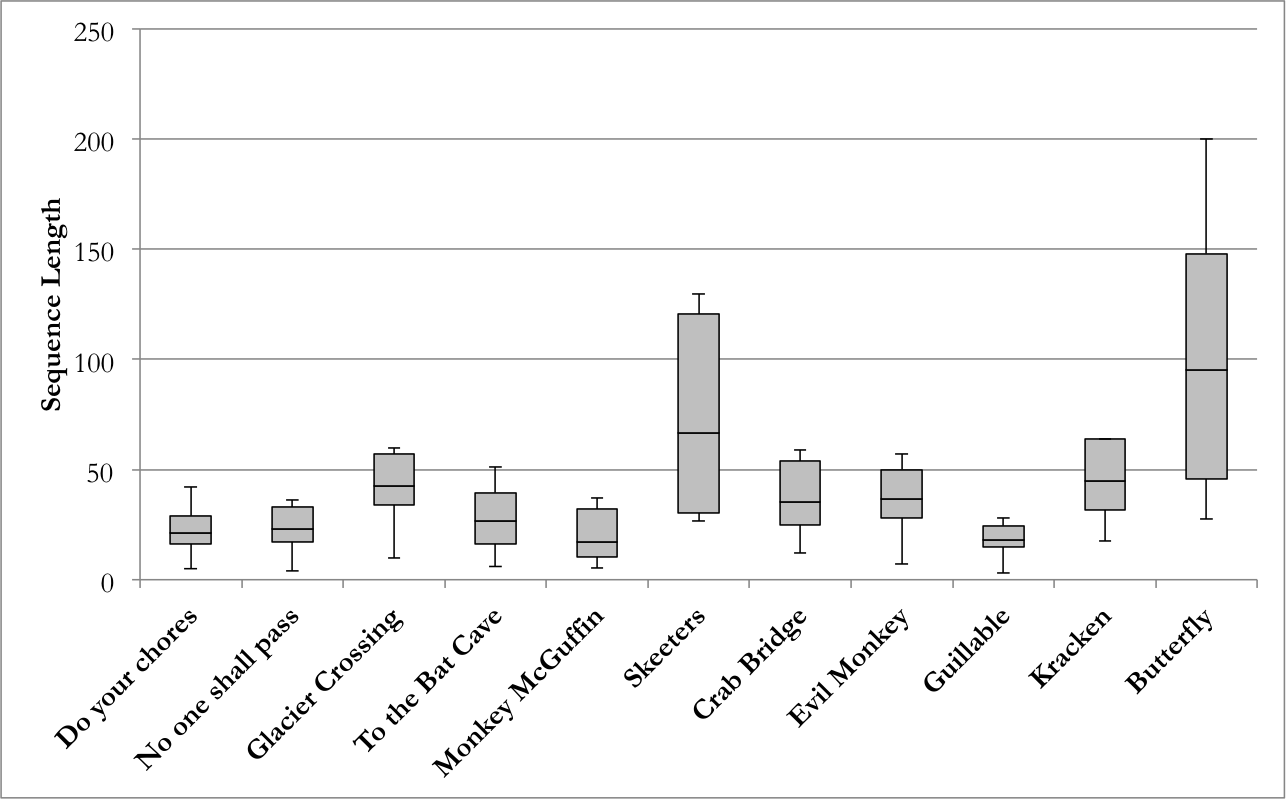
\includegraphics[width=0.9\columnwidth]{figures/boxplot}
	\caption{Boxplot of Sequence Length in Each Game Level}~\label{fig:boxplot}
\end{figure}

\subsection{Experimental Setup}
First we divide students into two groups, one (\%80) for training and development purposes and the other (\%20) for test and verification.
In the discretization phase, we transformed the log data from slot-and-filler structure each game level into sequences of multinomial variables that can be used as evidence for learning for each student.
In the sequence modeling phase, we use the multinomial sequences of students in the development set (\%80) to train two HMMs that that represent high- and low-performing students.
In the regression phase, we uses the likelihood of students' sequences in order to build a regression model that is predictive of the post-test results.
Finally, we test the regression model on the held-out set (\%20) and report the results.


\subsection{Results}
In order to evaluate our regression model we decided to compare its performance agains two baselines: 1) A regression model that uses success and failure of students in each game level as feature and 2) A regression model that uses the normalized sequence lengths in each game level. 
Our model was able to significantly outperform both baselines regarding to mean absolute error (MAE) and root mean squared error (RMSE). 
Moreover, the $R^2$ correlation and Spearman $\rho$ of our predicted values with the true values was much higher than both baselines. 
Table \ref{tab:results} shows the results. 

\begin{table}[tbh]
	\centering
	\begin{tabular}{@{}lllll@{}}
		\toprule
		\begin{tabular}[c]{@{}l@{}}\textbf{Predictive Features}\end{tabular}            & \begin{tabular}[c]{@{}l@{}}\textbf{$R^2$}\end{tabular} & \begin{tabular}[c]{@{}l@{}}\textbf{$\rho$}\end{tabular} & \begin{tabular}[c]{@{}l@{}}\textbf{MAE}\end{tabular} & \textbf{RMSE}\\ \midrule
		\begin{tabular}[c]{@{}l@{}}Sequence Length (Normal)\end{tabular} & 0.06                                                     & 0.79                                                 & 3.24                                                          & 4.15 \\
		Success / Failure                                                      & 0.01                                                     & 0.63                                                 & 3.22                                                          & 4.14 \\
		\algname                                                       & 0.55                                                     & 0.82                                                 & 2.84                                                          & 3.35 \\ \bottomrule
	\end{tabular}
	\caption{The results of predicting post-test scores using three different feature sets}~\label{tab:results}	
\end{table}

Figure~\ref{fig:regression} shows the true values vs. predicted values using LASSO regression along with the regression line and \%95 confidence interval.

The regression model also provides us with an insight into how important each game level is in distinguishing between high- and low-performing students. Table \ref{tab:regrweights} shows the weights of each game level in the best perfoming model.

\begin{table}[b]
	\centering
	\begin{tabular}{ll}
		\hline
		\textbf{Game Level} & \textbf{Weight} \\ \hline
		You Kraken Me Up!   & 1.686                               \\
		Skeeterz            & 1.059                               \\
		Evil Monkeys        & 1.053                               \\
		To the Bat Cave     & 0.855                               \\
		None Shall Pass     & 0.417                               \\
		...                 &                                    
	\end{tabular}
	\caption{Weights of each game level in the best performing model.}
	\label{tab:regrweights}	
\end{table}

As it is shown in the table, game level 11 (\textit{You Kraken Me Up!} -- screenshot Figure~\ref{fig:figurekracken}), has the highest weight in the regression model. This can be interpreted as the difference between the sequence of student interactions in this game level has the highest factor in distinguishing between high- and low-performing students. 

\begin{figure}
	\centering
	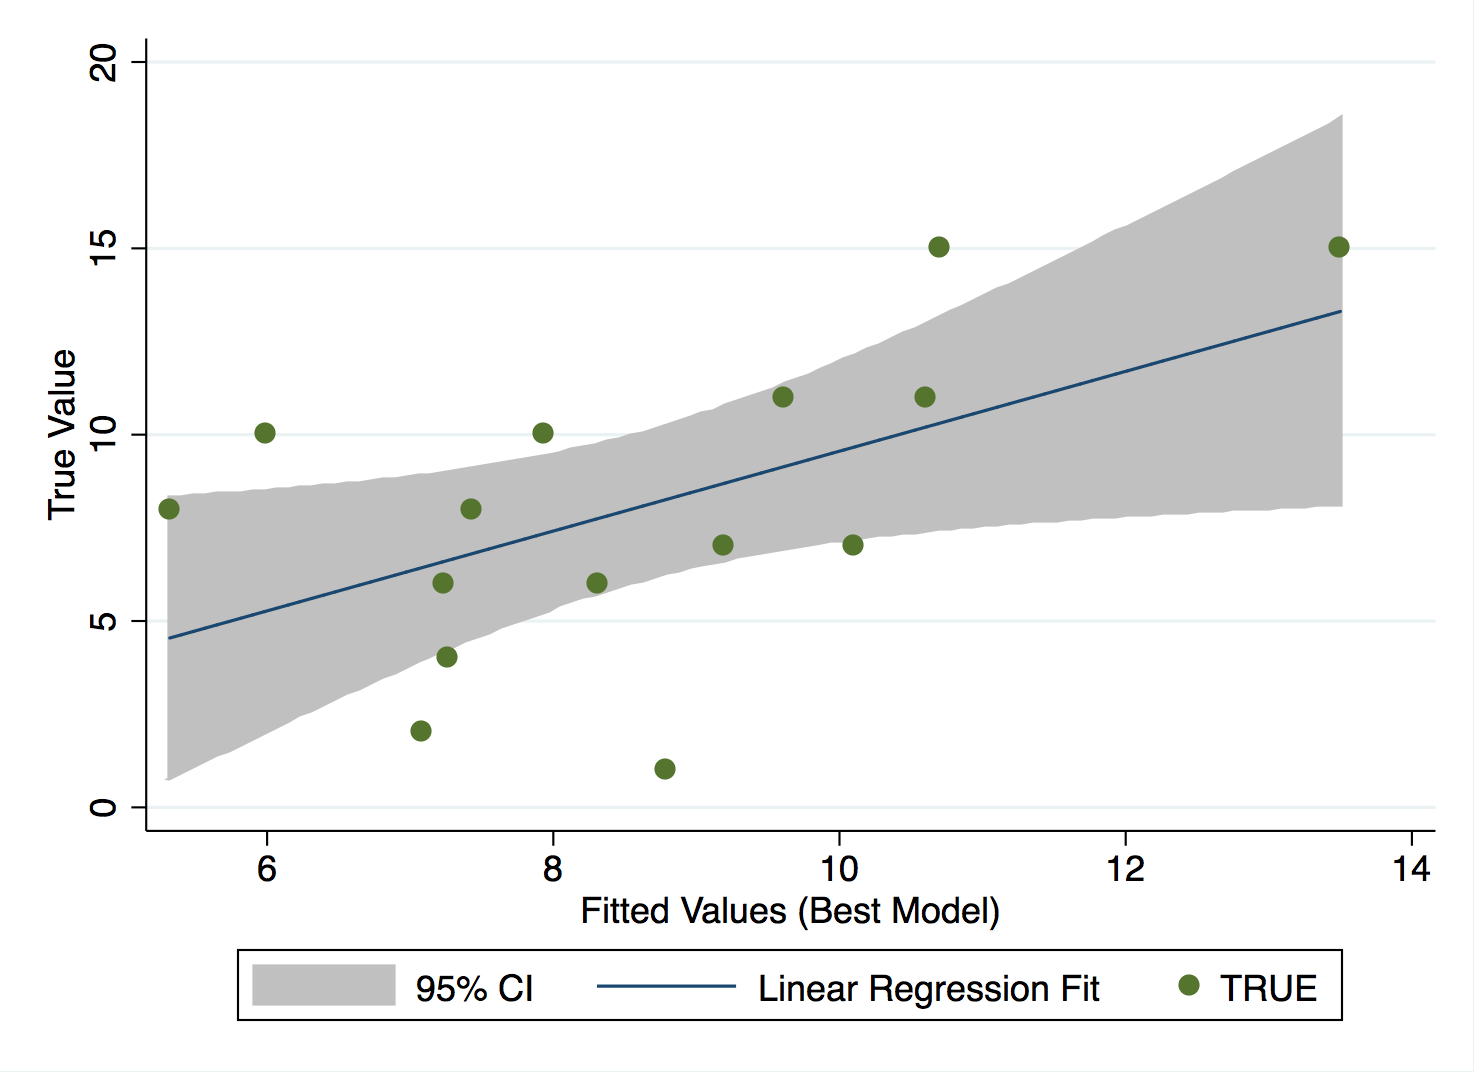
\includegraphics[width=0.9\columnwidth]{figures/regression}
	\caption{Results of predicting the post-test scores of the held-out set along with the regression line and \%95 interval.}~\label{fig:regression}
\end{figure}
	
\subsection{Discussion}
In this study we aimed to explore the effectiveness of data-driven methods for student modeling in educational games. 
To demonstrate the effectiveness of our framework, we used features from it to predict the post-test results using a regression model and showed significant improvement over two  baselines based on intuition. 
%The RMSE and MAE results, while significant, may not be the best metric to interpret the performance of our model since an improvement of 0.38 in MAE compared to the Success/Failure baseline means that on average our model  
\hl{Spearman correlation is the most important}
However, predicting post-test scores was not the only reason for designing the pipeline. 
We were also seeking for a descriptive model that can give us insight into low-level patterns in student movements. 
This was the main idea behind using HDP-HMMs in the sequence modeling phase and our hypothesis that high-performing and low-performing sudents have different sequential patterns. 

Figure~\ref{fig:highvslow} shows the difference between two HMMs learned for one of the game levels.
In this game level in the initial state, students are presented with composite objects and they have to use the \texttt{Esploda} tool to convert them into single unit objects. 
Then, they have to use the \texttt{Gluumi} tools to convert the single unit objects into composite objects that fit the designated area. 
And finally, they have to move the composite object they have created into the designated area.
For comparison purposes, we are showing a three state HMM for both high- and low-performing students and removed the edges that had the probability below 0.05. 
Figure~\ref{fig:highhmm} represents the HMM for high-performing students. The three latent states, $S_{0-2}$ can be interpreted as sequential steps, that students took for solving this problem. As illustrated in Figure~\ref{fig:highhmm}, high-performing students follow the expected path of using the \texttt{Esploda} tool in $S_0$, using the \texttt{Gluumi} tool in $S_1$, and then moving the composite objects into the designated areas \texttt{Move Combo\_{ClusterID}} untill they successfully finish the game.
On the other hand, low-performing students (Figure~\ref{fig:lowhmm}) do not necessarily follow the expected path and the probability of moving object into the outlier clusters (\texttt{Move Object\_0 and Move Combo\_0}) is also higher in each state for low-performing students.


% I CANNOT MOVE THIS FIGURE TO PAGE 6!!!!!
\begin{figure*}[t]
	\centering
	\begin{subfigure}{.5\textwidth}
		\centering
		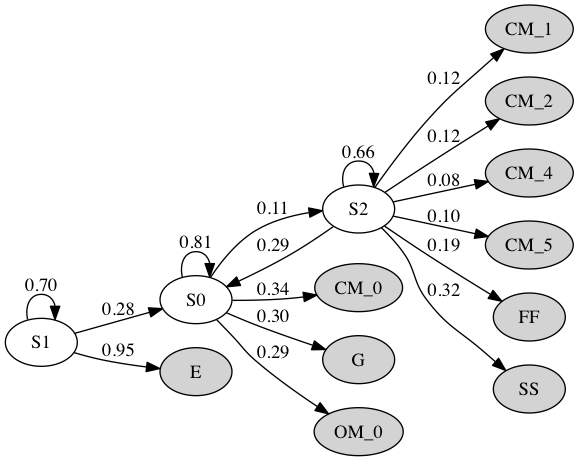
\includegraphics[width=0.9\columnwidth]{figures/high.png}
		\caption{High Performing~\label{fig:highhmm}}
	\end{subfigure}\begin{subfigure}{.5\textwidth}
		\centering
		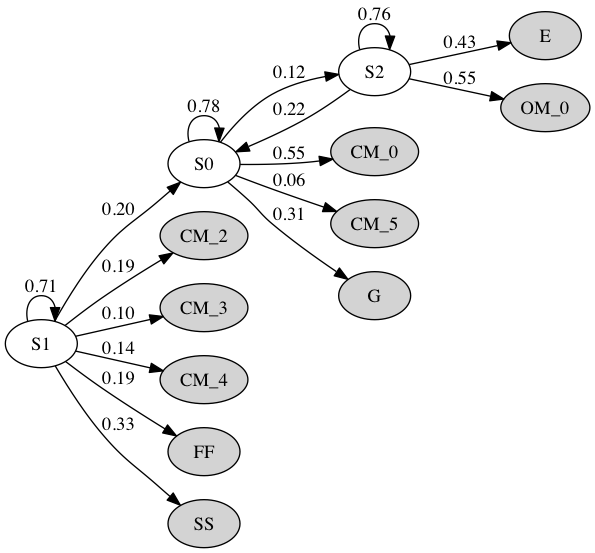
\includegraphics[width=0.9\columnwidth]{figures/low.png}
		\caption{Low Performing~\label{fig:lowhmm}}
	\end{subfigure}
	\caption{Two Hidden Markov Models learned from data in one of the game levels. The left HMM represents the high-performing students and the right one represents the low-performing ones.}~\label{fig:highvslow}
\end{figure*}

\section{Relation to Prior Work}
In order to deal with such highly unstructured data, researchers often use carefully designed network structures (such as Bayesian Networks \cite{albrecht1998bayesian,shute2013stealth}) or game-specific heuristics and benchmarks generated by experts playing the game \cite{mandel2014offline,tastan2011learning}. However, this approach is extremely labor intensive and might fail to capture meaningful patterns in student exploratory habits within the game. Given these limitations, data-driven analysis of student interactions provides a powerful alternative that facilitates the discussions around what does and does not work in a particular educational game.

The potential of computer games for educational purposes has been of interest since nearly the beginning of videogames. Unlike video games, which focus on creating an entertaining experience for the user, educational games require principles and strategies that engage students while maximizing their learning gain. Therefore, data-driven analysis of student behavior is crucial to better understand the learning process and improve the tools in the future.

There have been numerous attempts among the educational research community to develop analytic methods and build predictive models based on the data from educational games. \textit{Newton's Playground} is an ECD based educational game with 74 problems that designed to teach qualitative physics to students in eighth- and ninth-grade. Students have to guide a green ball to a red ball by creating simple machines. 
Everything obeys the basic rules of physics relating to gravity and Newton’s three laws of motion. 
Shute et al. \cite{shute2013stealth} studied the effect of ECD design on student learning and found that students who played the game in a 4 hour session, showed significant improved in their qualitative, conceptual physics understanding.

\textit {Rumble Blocks}  is another educational game designed to teach basic concepts of structural stability and balance to children in grades K-3 (ages 5-8 years old). Harpstead et al. \cite{harpstead2014using}, studied the alignment of game to its target learning goals by examining whether student solutions follows the targeted principals. They employ clustering techniques on the individual solutions created by actual students and use principle-relevant metric (PRM) to measure how closely the representative solution embodies a specific targeted principle. The results demonstrated a misalignment between the feedback provided to students and the targeted knowledge.

\textit {Battleship Numberline} is another educational game for understanding fraction using number line estimation. Students attempt to explode target ships and submarines by estimating numbers on a number line. Lomas et al. \cite{lomas2013optimizing} performed a large-scale online experiment in order to study the effect of challenge on player motivation and learning. They presented different configurations of the game for different groups of students and used a combination of time spent and challenges attempted as a measure of engagement and the average success rate of each design configuration as a measure of challenge. The results showed a linear correlation between challenge (difficulty) and engagement, meaning the easier the game, the longer students played.

\textit {Refraction} is another educational game for learning about fractions by splitting laser beams into fractional amounts to target spaceships by avoiding asteroids. Liu et al. \cite{liu2013predicting}, created an ensemble algorithm that combines elements of Markov models, player heuristic search, and collaborative filtering techniques with state-space clustering in order to predict player movements on last game-level based on the history of movements in previous game levels. Lee et al. \cite{lee2014learning} extended the former framework by building state-action graph and using feature selection techniques to reduce the number of features for each state. To ensure extensibility, they also tested the framework on another game \textit {DragonBox} and reported improvement over a Markov predictor.

\section{Conclusion}
Modeling student behavior in open-ended environments such as educational games is an interesting and complex problem. Particulary data-driven models, can be valuable tools for game designers, educators, and researchers for analyzing how students learn different skills by using their systems.
In this paper, we presented a data analysis framework that is able to learn a model from game activity logs that is predictive of student proficiency with minimum reliance on expert knowledge about the game environment. 
One of the key drawbacks of model-free methods is that their results are difficult to interpret. 
However, the discretization process along with the use of HDP-HMM, makes our model human readable and can give us insight into how student interact with each game level.
Moreover, the parameters of the regression model provides a good intuition about the importance of each game level and its influence in distinguishing between high- and low-performing students.

There are many possible directions for future work. On a lower level we can integrate the discretization and sequence modeling step by designing a new type of Hidden Markov Model that accepts slot and filler sequences as input (work in progress). On a higher level, instead of dividing students into two groups (high- and low-performing), we can use the new type of HMM in order to cluster students into more groups that might be  more representative of different approaches students follow in order to solve each game level. We can also replace our regression model with a more powerfull ensemble method that considers different subskills in order to integrate features of each game levels in order to predict the post-test scores.

We only used data from \textit{Alice in AreaLand} in order to evaluate our model. However, the model is designed in a way that can model sequence of student actions in other similar gaming environments that use slot-and-filler structures in order to log student interactions with the system. Finally, using our framework we will be able to build a model that detects incorrect strategies or common misconception that can be used in a dynamic hinting system in order to increase player engagement and learning. 

\hl{Limitation, we don't compare to Valerie Schultz}

\hl{Limitation, we don't control for game ability like Valrerie does}

\hl{Limitation, we only used data from Alice in wonderland}

\hl{Method is accuaate}


\bibliographystyle{SIGCHI-Reference-Format}
\bibliography{references}

\end{document}
